
% Many thanks to Andrew West for writing most of this file
% Main LaTeX file for CIS400/401 Project Proposal Specification
%
% Once built and in PDF form this document outlines the format of a
% project proposal. However, in raw (.tex) form, we also try to
% comment on some basic LaTeX technique. This is not intended to be a
% LaTeX tutorial, instead just (1) a use-case thereof, and (2) a
% template for your own writing.

% Ordinarily we'd begin by specifying some broad document properties
% like font-size, page-size, margins, etc. -- We have done this (and
% much more) for you by creating a 'style file', which the
% 'documentclass' command references.
\documentclass{sig-alternate}
 
% These 'usepackage' commands are a way of importing additional LaTeX
% styles and formattings that aren't part of the 'standard library'
\usepackage{amsmath}
\usepackage{mdwlist}
\usepackage{url}
\usepackage{float}
\usepackage{listings}

\begin{document} 

% We setup the parameters to our title header before 'making' it. Note
% that your proposals should have actual titles, not the generic one
% we have here.
\title{Programming Language Support for Probabilistic Associative Memory}
\subtitle{Dept. of CIS - Senior Design 2014-2015} %\thanks{Advisor: Steve A. Zdancewic (stevez@cis.upenn.edu).}}
%\thanks{ Do not list your advisors amongst the authors as that may cause Google Scholar to add this work to their list of publications. Your advisor must also sign a hard-copy of your proposal.}}
%\thanks{ }}
\numberofauthors{3}
\author{
    Fan Yin \\ \email{fanyin@seas.upenn.edu} \\Univ. of Pennsylvania \\ Philadelphia, PA
    \and Haolin Lu \\ \email{haolinlu@seas.upenn.edu} \\Univ. of Pennsylvania \\ Philadelphia, PA
    \and Yukuan Zhang\\ \email{yukuan@seas.upenn.edu} \\Univ. of Pennsylvania \\ Philadelphia, PA
}
%\author{
%\alignauthor Radoslav Ivanov \\ \email{rivanov@seas.upenn.edu} \\ Univ. of Pennsylvania \\ Philadelphia, PA 
%
%\and Radoslav Ivanov \\ \email{rivanov@seas.upenn.edu} \\ Univ. of Pennsylvania \\ Philadelphia, PA 
%
%}
\date{}
\maketitle

% TODO: don't mention ocaml except in system implementation.
% TODO: get rid of "we"?
% TODO: Figure re-numbering
% TODO: references/bibliography

% Next we write out our abstract -- generally a two paragraph maximum,
% executive summary of the motivation and contributions of the work.
\begin{abstract}
    Our goal is to create a programming language library that provides an interface
    for programming with a probabilistic associative memory.
    A probabilistic associative memory receives an input and returns a value associated with
    or similar to the input. This project provides an intuitive interface to this probabilistic
    associative memory to facilliate programming efficiency for the end user. It will primarily
    accomplish this by providing an easier way to handle structured input data for the user, as well
    as automatically managing user-defined types in memory.
\end{abstract}

\section{Background}
\label{sec:intro}

The standard way to access a stored value in memory is by address. 
This involves finding the physical position of that address in memory
and returning the stored value. Meanwhile, associative memory allows
searching for values based on the stored content. An analogous structure
in programming languages is the hashtable, which returns an output value
based on an input key. 

Standard associative memories are useful for when one needs to query memory based 
on some input data or tag. For instance, router firmware often employs associative 
memories to store tables of Internet Protocol (IP) addresses, which serve as the ``next hop" for incoming 
packets. Since routers looking for the ``next hop" have a specific, standard query 
format -- e.g. an IP address of the form www.xxx.yyy.zzz -- it makes sense to store the 
routing tables based around this input string.

Probabilistic associative memories retain the content-based characteristics of associative memories.
However, they stop maintaining the one-to-one relationship between input and output.
A modern day realization of probabilistic associative memories is the neural network. A neural network
consists of a series of functions acting on ``features" or characteristics of given input values. Using
these functions, it can find relationships or make predictions on its inputs. It also
reacts and changes whenever it sees new input to enhance accuracy for future input.

Neural networks are a small part of the much broader topic of \textbf{machine learning}. Machine learning
is widely used today to solve problems that lack easily definable patterns (i.e. natural language processing,
computer vision, classification). A common feature of these problems is that they usually have a large amount
of sample data available. The goal of machine learning algorithms is to build models based on an
abundant amount of ``training data". Since the types of data vary wildly from one problem to the next,
from sentences in several languages to video data from a camera, a way to reconcile the data with
mathematical models is required. In this respect, ``feature extraction" is essentially the de facto
standard for a majority of machine learning algorithms. Feature extraction involves transforming the
input data into a vector of real numbers, while trying to encapsulate as much of the information
in the original data as possible. These vectors are then run through the model to improve accuracy,
acquire a result, or both. Figure \ref{fig:mlworkflow} is a representation of this process as
applied to a classification problem in machine learning. 

%See Figure 1 for a representation of the flow of this probabilistic mechanism.
\begin{figure}[h]
	\begin{center}
		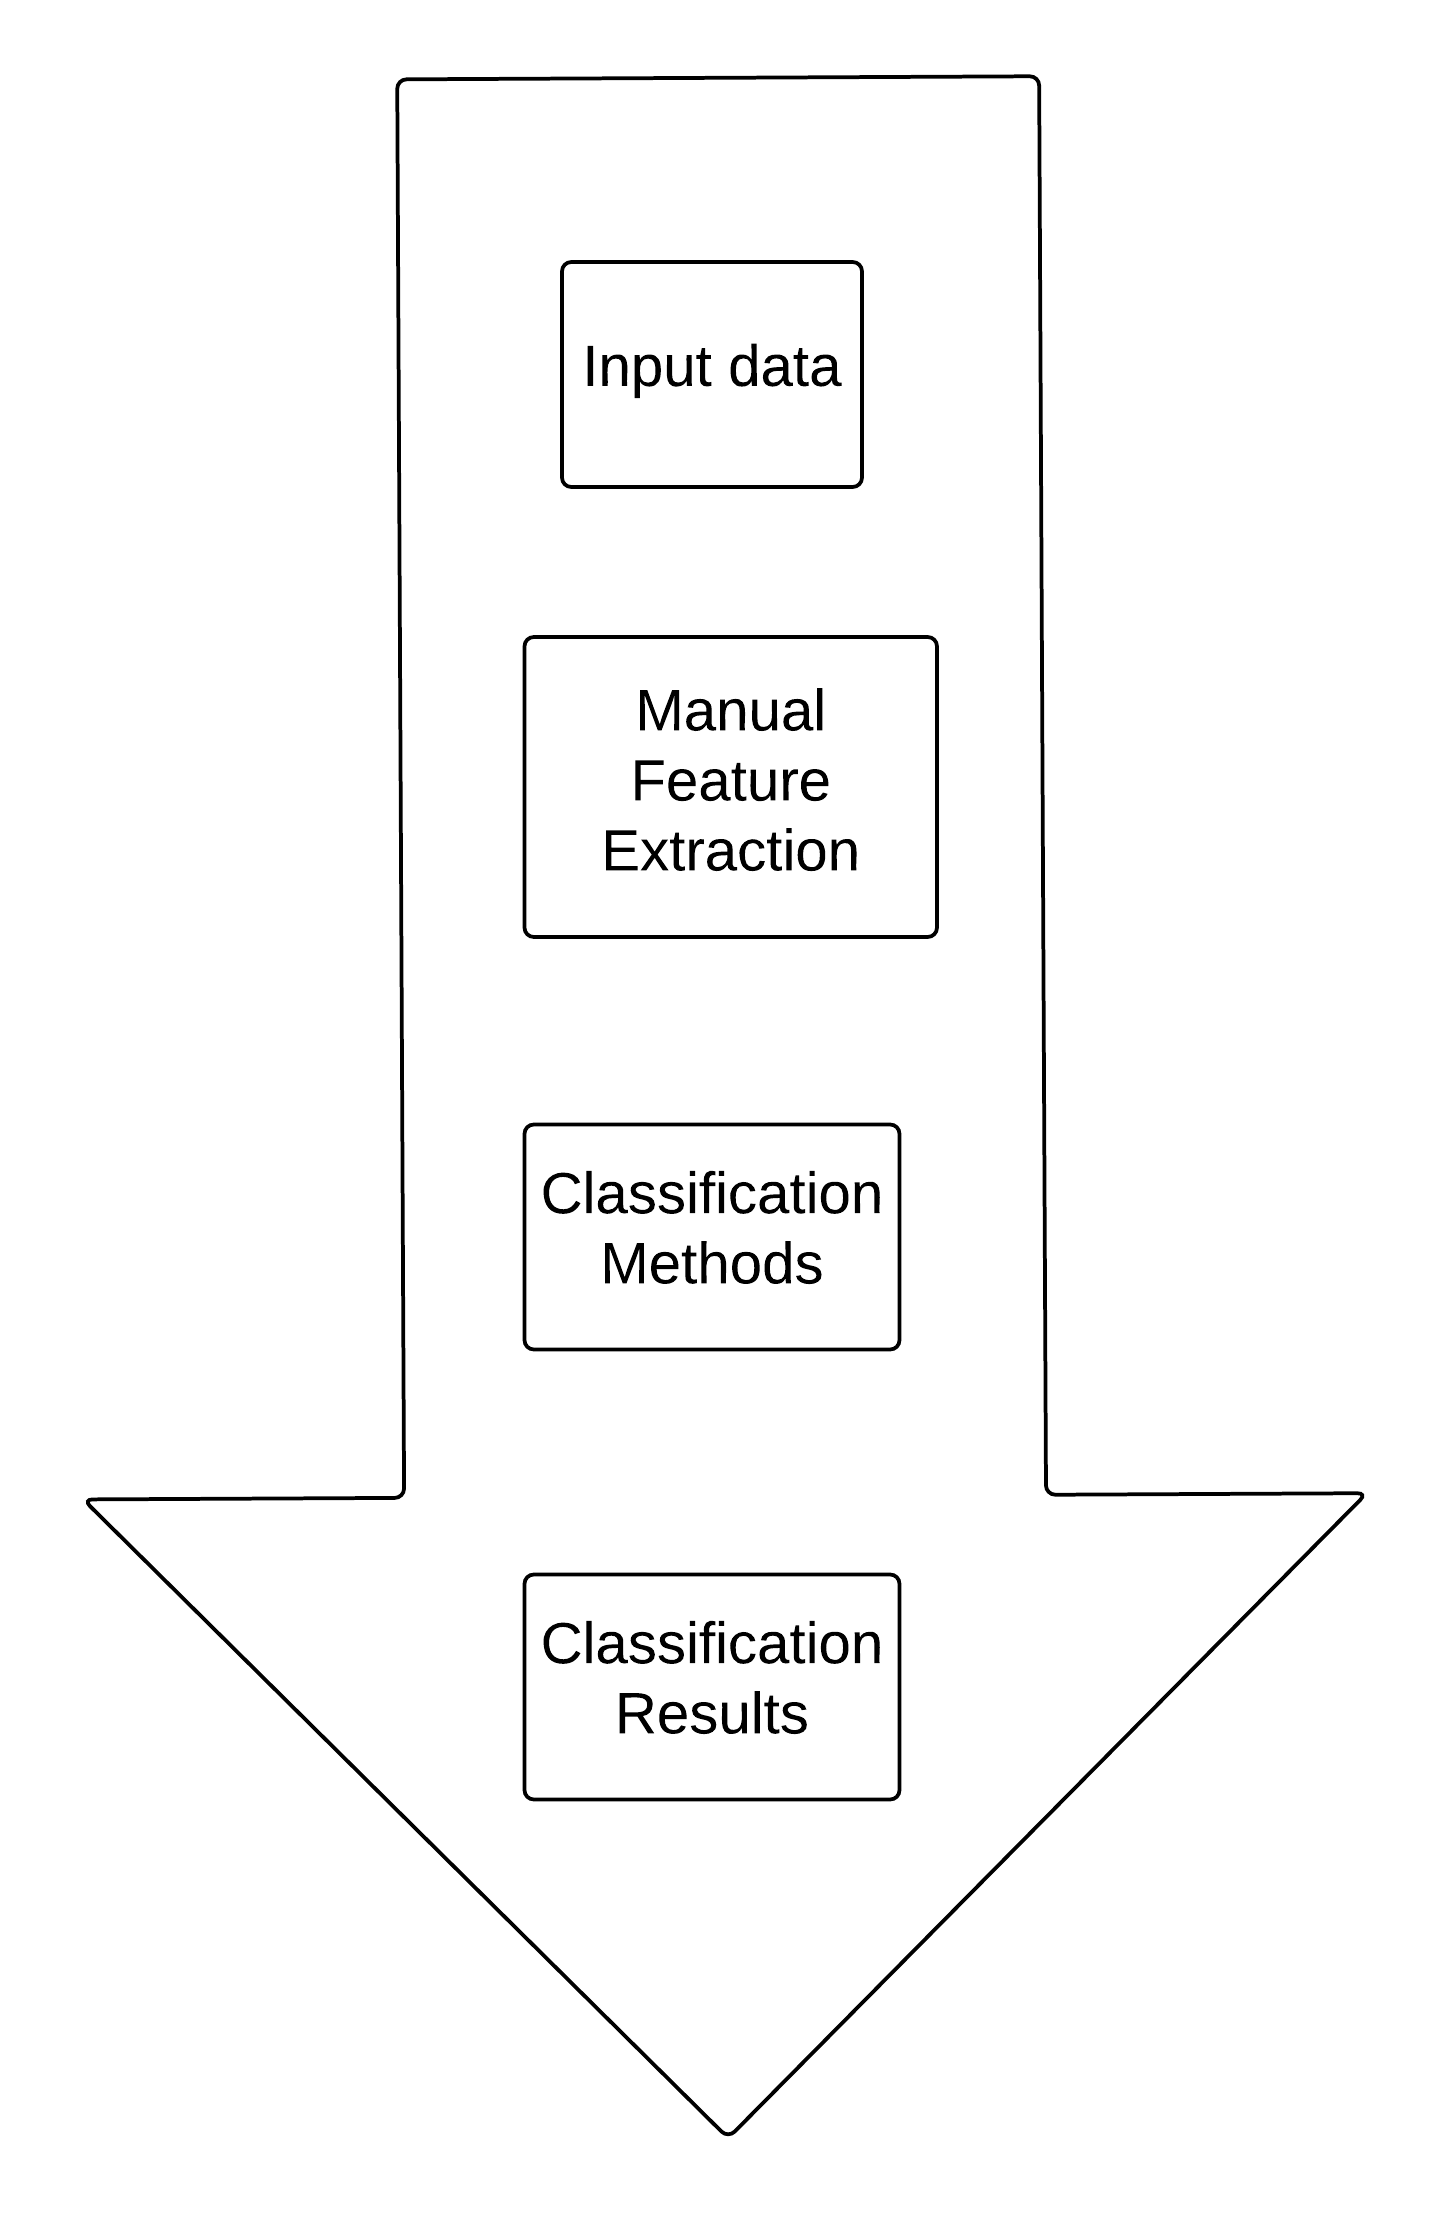
\includegraphics[width=0.75\linewidth]{mlworkflow}
	\end{center}
	\vspace{-12pt}
	\caption{Model of Standard Machine Learning Workflow}
	\label{fig:mlworkflow}
\end{figure}

The autoencoder and kernel methods are specific methods in machine learning that aid with feature
extraction. Autoencoders are neural networks that take in a set of data and return a reduced, 
compressed representation of that data. That is, it returns an encoding that represents the qualities of
the original data as faithfully as possible. This is akin to feature 
extraction, since the whole concept of feature extraction is finding the essential features 
of a set of data. As shown in Figure \ref{fig:kernelmeth}, kernel methods are a way of projecting
a set of data in one space to another space, with the intention that it may
be easier to extract and separate essential data in the latter space. As shown in the figure, the
points on the $xy-$plane are not separable with a hyperplane, but when projected into three 
dimensions, they are more easily separated, and thus easier to classify into ``red" and ``blue" 
categories. If ``red" and ``blue" are thought of as separate features, then it is apparent to see
how kernel methods aid in classifying features of a dataset. Notably though, kernel methods can
also increase the dimensionality of the data, in the hopes that the new feature space is more 
descriptive than the old. 

\begin{figure}[h]
	\begin{center}
		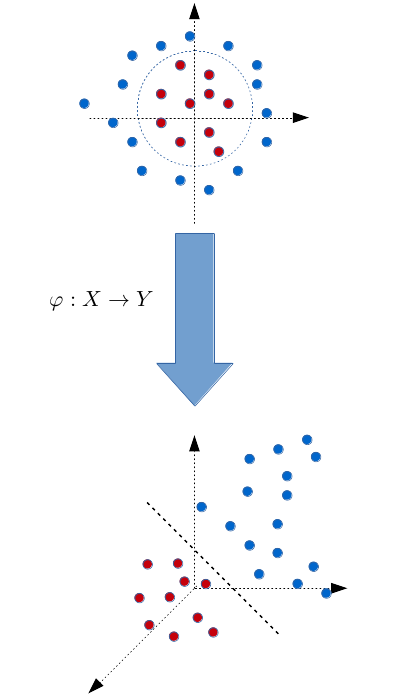
\includegraphics[width=0.75\linewidth]{kernelmeth}
	\end{center}
	\vspace{-12pt}
	\caption{Representation of Kernel Method}
	\label{fig:kernelmeth}
\end{figure}

Machine learning ideas and techniques will be crucial to this project. 
They will be used as the foundation of the memory system. It will also be the field where this 
project will have the biggest impact.

\section{Introduction}
\label{sec:intro}

In machine learning, the process of obtaining features from data is dependent upon
the type and structure of the data. While for certain things like strings or images
will have features such as word count or pixel value, structured data such as lists, pairs, 
trees, or other types of data structure can potentially be much more complicated due to the
recursive nature of lists and trees.

Handling this issue with structured data of any generic type is an important feature of the 
programming language library, and various methods of this genericized feature projection have been 
investigated. Since these methods are intended to be applied on top of the probabilistic
associative memory, work on the memory backend of the library interface has also been accomplished.

Moreover, after features are obtained, feature extraction to reduce the set of descriptive
features is generally necessary. This is especially necessary for structured data 
inputs, as features are created to describe not only the content, but the structure of the data.

What must still be done is integrating these extraction methods with the library interface.
As will be detailed later, there has been research done on linear autoencoders
for structured data, and there has also been previous work on convolution 
kernels for natural language processing -- a field that processes a lot of 
data in the form of structured trees. The mathematical machinery behind autoencoders and kernel 
methods will thus be investigated further and they must eventually be implemented in the library.

In the next section, the paper will proceed by delineating works related to 
associative memories and will go more in-depth about autoencoders 
and convolution kernels. Then, it will establish a model or workflow of the 
library interface, and the process of using this interface for machine
learning applications. After that, it will go into some details of the library
implementation, discuss the choice of language and present some third-
party libraies that were used. Finally, the performance of the current
implementation will be discussed, as well as more details regarding the remaining work.

\section{Related Work}
\label{sec:related_work}

With regards to existing related work, the goal of this project is not to advance associative memory 
techniques. Rather, it is seeking to research existing models for associative memories, provide a 
simple probabilistic query interface, and integrate a method of extracting essential features from 
the structured data that is input into the memory. With that in mind, there are many works that 
address associative memory and feature extraction from structured data.

Research in associative memory has close connections to neural networks. Our brains function as 
associative memories that can retrieve memories based on similarity between stimuli and the memories 
themselves.  Indeed, Norman and Bobrow~\cite{bobrow} construct a memory model which describes how 
minds retrieve items in memory from partial descriptions, even if some part of the description is 
incorrect or inaccurate. 

Applying this memory model to computation, Hinton~\cite{hinton} draws a connection between Norman 
and Bobrow's idea of retrieving memories based on partial descriptions and content-addressable 
memories.  Hinton then notes that although this content-addressable memory is a useful 
representation, it is difficult to efficiently ``search for content" through a memory space. 
Hinton ends by claiming that while this model is conceptually not difficult, it is difficult to 
actually implement it. He mentions that an approach to this problem that has arisen recently is with 
stochastic processes -- heralding a probabilistic approach to this associative memory problem.

Hinton's issue of search efficiency is related to the size of the data sets that
one would feed into a neural network.  To address the issue of increasingly large data sets, 
resulting in larger and larger feature vectors, much research has been made to decrease 
dimensionality of feature vectors. An early but effective technique is principle component
analysis, or PCA, which utilizes matrix operations and covariance of features to ensure
that the reduced dimensionality feature space is as representative as possible of the original
feature space. A more modern technique introduced earlier is the autoencoder, which performs a
similar dimensionality mapping, but using neural network techniques. Researchers Hinton 
and Salakhutdinov~\cite{autoencoder} describe a method of creating deep autoencoders to learn low 
dimensionality codes that maintain high fidelity with respect to codes of the original dimension.

\begin{figure}[h]
	\begin{center}
		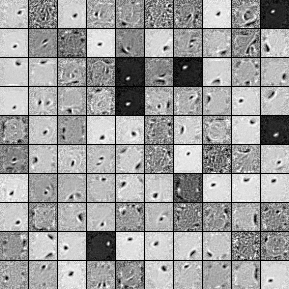
\includegraphics[width=0.75\linewidth]{filters_corruption_30.png}
	\end{center}
	\vspace{-12pt}
	\caption{Features extracted from pictures of single digits}
	\label{fig:features}
\end{figure}

As an example - figure \ref{fig:features} is a set of features for pictures of handwritten single 
numerical digits (0-9) from the MNIST dataset, a dataset with 60,000 training examples
and 10,000 test examples~\cite{denoise}. All of the examples have been normalized in size and position, as well as 
color. Due to the preprocessing, it is commonly used in machine learning for testing out learning 
techniques on real world data.  These features were extracted from a simple one-layer autoencoder, 
which manages to capture small regions of the input image as "features". 

An extension of classic autoencoders called a denoising autoencoder has the ability to reconstruct 
partially missing or corrupt inputs. This property of denoising autoencoders make them extremely 
promising for use in a memory system. Like classic autoencoders, 
denoising autoencoders work by passing input through a hidden 
layer, a matrix that represents a transformation, to encode it in a lower dimension. The original 
input is then ``retrieved" by doing a reverse transformation on the encoded version.~\cite{denoise}

While a denoising autoencoder acts as an effective probabilistic associative memory, it is
limited by the fact that it works only on vectors as input. There are many cases in machine
learning, in fields such as bioinformatics and natural language processing where it would be 
extremely useful to represent data in a structured form, rather
than converting it to feature vectors. In relation to this, Alessandro Sperduti~\cite{sperduti}
found a way to create linear autoencoder networks for structured data, specifically
arbitrary sequences and trees. The idea is that linear autoencoder networks are actually
closely linked to PCA. By using this connection and modeling the structured data via
linear dynamical systems, Sperduti was able to create a way to store structured data
in an autoencoder network.

A comlementary technique to that of Sperduti is kernel methods. Kernel methods refers to the
use of a kernel function to preprocess input to make it easier for certain algorithms to run. 
While kernel methods exist for a vast array of problems and data sets, Collins and Duffy~\cite{kernels}
created a method called convolution kernels for natural language processing. In natural
language processing, one often deals with parse trees as input data, and this kernel technique
represents another way for structured data to be used with other standard machine learning
algorithms, such as autoencoders.

\section{System Model}
\label{sec:sysmodel}


%TODO: talk more about the memory?
Figure \ref{fig:ourworkflow} shows a model of the workflow of using this programming library, as 
used for machine learning. In similar fashion to standard machine learning applications, the user 
will start with a set of training data which can take various structures such as trees or lists. The 
user will then need to specify the type and structure of the data he is inputting to the library, so 
the library will know how to process it appropriately. 


%FIGURE: Standard flow for this library implementation
\begin{figure}[h]
	\begin{center}
		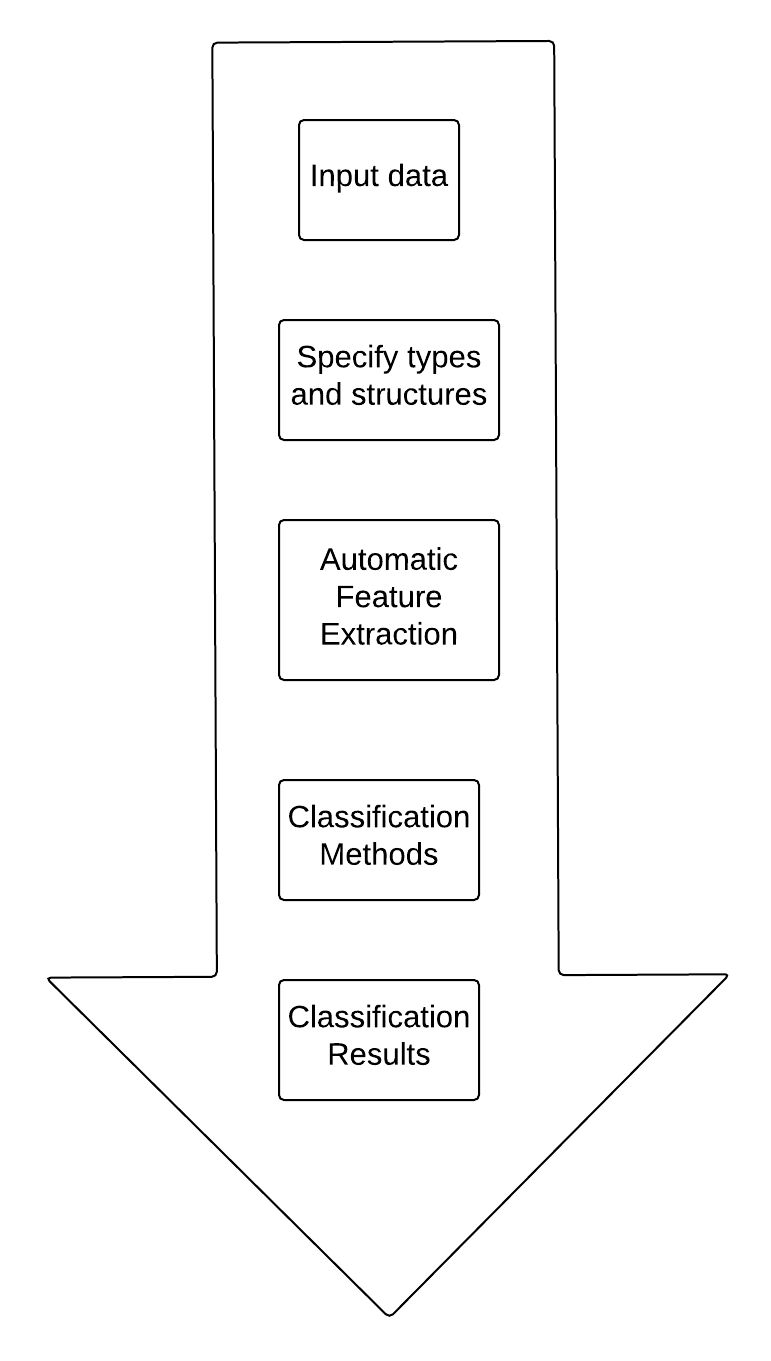
\includegraphics[width=0.70\linewidth]{ourworkflow}
	\end{center}
	\vspace{-12pt}
	\caption{Library Interface Workflow as Applied to Machine Learning}
	\label{fig:ourworkflow}
\end{figure}

\vspace{10pt}

Regarding this data specification, the user will do this implicitly when he processes 
his sample data and loads it into custom types defined by the library or by OCaml itself. 
Next, the library will use an algorithm or model to actually perform this feature extraction. In 
comparison to the standard machine learning workflow in Figure \ref{fig:mlworkflow}, the workflow 
when using this library will provide automatic feature extraction, as opposed to requiring the 
programmer to manually extract the feature through his own custom code.  The rest of the library 
after feature extraction will more or less proceed according to standard machine learning methods.
That is, the library will run the vectors through classification algorithms and models 
and return the classification results or decisions to be used on actual, untrained data.

As stated before, there is literature on machine learning methods that handle ``automatic" feature 
extraction, given the type or structure of the data. Recall that convolution kernel methods and 
linear autoencoder networks could accomplish this extraction over various structures of data. These 
methods have been tested and applied to NLP applications and classification problems involving data 
stored in trees and sequences.  Thus, the approach of this library should at least work for any sort 
of tree-like or list-like structure.

\section{System Implementation}
\label{sec:sysimp}

In order to implement a generalized process for handling structured data, the programming language 
library has been written in OCaml. OCaml is a functional language, so it will be more fluid to use 
when handling structured data. In addition, OCaml has procedural elements that facillitates the ease 
of implementing and prototyping the various algorithms and models that have been encountered so far. 
Regarding third-party libraries, there is a linear algebra for OCaml called Lacaml that uses BLAS 
(Basic Linear Algebra Subprograms)
and LAPACK (Linear Algebra PACKage)
as its backend, which are two well-established, robust and performant linear algebra 
libraries. Notably, the low-level BLAS is widely used in scientific computation in many more complicated
higher level packages, such as MATLAB or R. 

In terms of the query interface, it currently contains all the functionality needed for basic 
queries.  This includes the basic ``wildcard" and ``constant" queries, as well as support for 
``pair" and ``either" queries. This was created using the standard OCaml interface setup. In the 
future, extra queries will be needed to deal with structured data, but the interface will be easily 
extensible due to the flexible type system of OCaml. The interface also has the ability to use 
different types of underlying mechanisms as a memory (Figure \ref{fig:queryint}).

%FIGURE: Standard flow for this library implementation
\begin{figure}[h]
	\begin{center}
		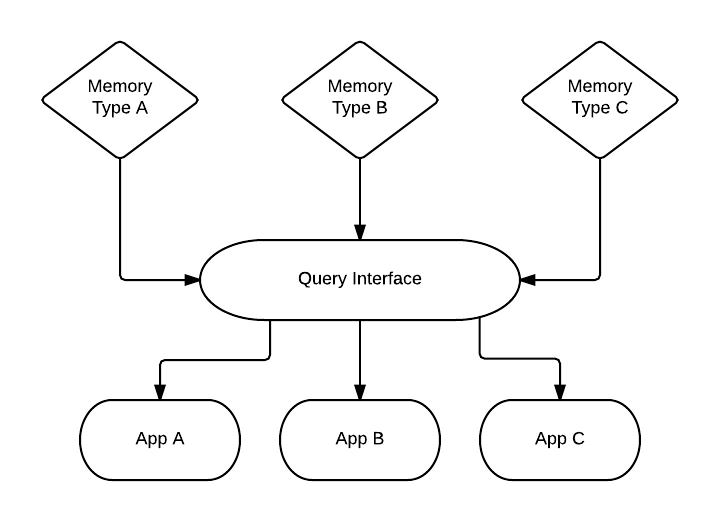
\includegraphics[width=1\linewidth]{queryint}
	\end{center}
	\vspace{-12pt}
	\caption{Query Interface of Library}
	\label{fig:queryint}
\end{figure}

One possible type of memory using the autoencoders discussed in the related work
section has already been implemented. An autoencoder uses hidden layers (matrices) to perform 
transformations on input vectors, compressing them to a lower dimension and doing a reverse 
transformation to retrieve them. 

Let $x$ be the input vector. As shown in Equation 1, $x$ can be transformed to a lower dimension 
vector $y$ by applying a transformation matrix $W$ and adding a bias value $b$, then applying a non-
linear transformation $s$, such as the sigmoid function.

\begin{gather}
y = s(Wx + b)
\end{gather}

It can then ``retrieve" the original value by applying reverse transformations to $y$, using
a different matrix $W'$ and bias factor $b'$, as shown in Equation 2.

\begin{gather}
z = s(W' y  + b')
\end{gather}

Finally, it learns the correct matrices by comparing the input value $x$ to the retrieved value $z$ 
using the cross-entropy error rate $L(x,z)$, and adjusting appropriately, as shown in Equation 3.

\begin{gather}
L(x,z) = -\sum_{k=1}^d [x_k \log z_k + (1-x_k) \log( 1-z_k)]
\end{gather}

Notice that as the dimensionality
of the hidden layer increases, the optimal transformation matrix approaches the identity, since
the identity matrix is the best possible representation if the hidden layer had the same dimension
as the input. To create useful representations even in these situations, the autoencoder is trained
by intentionally corrupting the input, passing it through the autoencoder, and doing a gradient
descent on the error between the output and the original input. That is, the error is differentiated
with respect to the weight matrix $W$ and the bias value $b$, and $W$ and $b$ are then updated in the
direction of decreasing error. This trains the autoencoder
to be able to reconstruct partially missing input, as is the goal of the query interface.

\section{System Performance}
\label{sec:sysperformance}

The portion of the library that can be measured so far is the basic autoencoder model. 
Since it is based on a reference implementation, performance statistics of both
implementations can be compared. Due to randomization inherent in the algorithm, however, 
performance must be standardized by either choosing the same random initialization parameters, or 
averaging across multiple runs. 

At the moment, substantial tests are not possible due to performance issues in the current 
implementation. Initial manual tests with set parameters and tiny data points seem to heavily favor 
the existing implementation with respect to performance. This is likely due to the gradient descent
method used. While concrete tests of actual data sets have not 
been run, test runs of the reference implementation have been run locally. A chart of runtime
performance for those runs is provided, as well as estimated performance of our current 
implementation given the small manual tests run(Figure \ref{fig:performance}). 

\begin{figure}[h]
	\begin{center}
		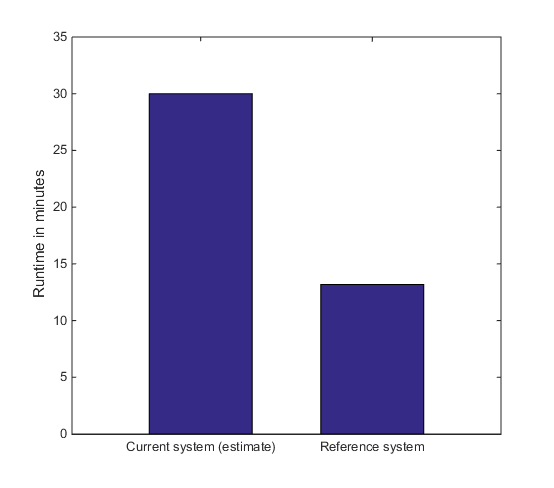
\includegraphics[width=1\linewidth]{performance.png}
	\end{center}
	\vspace{-12pt}
	\caption{Estimated runtime performance of current implementation and runtime performance of reference implementation}
	\label{fig:performance}
\end{figure}

This reference implementation is run on the MNIST dataset.
Regarding accuracy, it seems that our current implementation suffers from a bit of inaccuracy
when compared to the reference implementation. This is likely due to the symbolic math
package used in the Python-based reference implementation, which can defer calculations
and perform symbolic differentiation, resulting in higher accuracy. Since only
small manual tests have been run, the following chart (Figure \ref{fig:error}) of cross-entropy error is with just the
reference implementation error. 

\begin{figure}[h]
	\begin{center}
		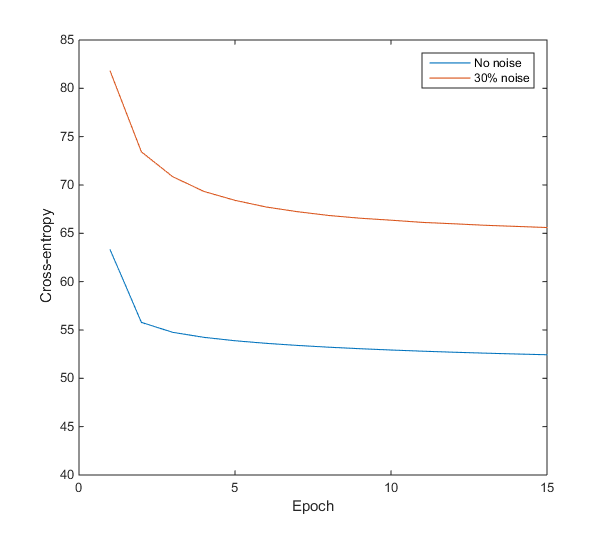
\includegraphics[width=1\linewidth]{error.png}
	\end{center}
	\vspace{-12pt}
	\caption{Cross-entropy error of target implementation}
	\label{fig:error}
\end{figure}

\section{Remaining Work}
\label{sec:project_proposal}

Currently, a basic autoencoder model has been implemented, and a specification of the library's
interface, as well as a simple test implementation of the interface, has been created. 
However, the autoencoder model is still far from finished. The most immediate improvement
that can be made is to improve the performance of the basic autoencoder model. Since the gradient
descent method being used is currently hand-written in OCaml, it seems that increasing 
performance may require linking to external libraries. However, it still may be possible to
optimize the current method, which would be preferable in order to keep as much of the 
implementation in OCaml as possible.

Next, provided that the gradient descent method used is optimized, the autoencoder model will 
need to be built into a multi-layer autoencoder for accuracy. This introduces a significant
amount of additional complexity, although the basic model will still be the foundation for
the multi-layer model. 

The most challenging task remaining will be to utilize the structured data kernels in order to
provide structured data support. While methods have been written and published on paper,
this is still unexplored territory regarding implementation. This portion alone will likely 
represent over half of the remaining work due to its complexity and relative novelty. 

Performance will likely continue to be an issue throughout the remaining tasks, due to a lack
of library support for the methods that will be implemented. Thus, it is likely that while 
this library will be able to accomplish its goals, it may not be as performant as existing 
libraries. However, there are few libraries even in existence, so this library will hopefully
be impactful regardless. 

% We next move onto the bibliography.
\bibliographystyle{plain} % Please do not change the bib-style
\bibliography{progress_spec}  % Just the *.BIB filename
% Here is a dirty hack. We insert so much vertical space that the
% appendices, which want to begin in the left colunm underneath
% "references", are pushed over to the right-hand column. If we looked
% hard enough, there is probably a command to do exactly this (and
% wouldn't need tweaked after edits).
\vspace{175pt}

\end{document} 

